\documentclass[12pt,letterpaper,fleqn]{hmcpset}
\usepackage[margin=1in]{geometry}
\usepackage{graphicx}
\usepackage{amsmath,amssymb}
\usepackage{enumerate}
\usepackage{hyperref}
\usepackage{parskip}

% Theorems
\usepackage{amsthm}
\renewcommand\qedsymbol{$\blacksquare$}
\makeatletter
\@ifclassloaded{article}{
    \newtheorem{definition}{Definition}[section]
    \newtheorem{example}{Example}[section]
    \newtheorem{theorem}{Theorem}[section]
    \newtheorem{corollary}{Corollary}[theorem]
    \newtheorem{lemma}{Lemma}[theorem]
}{
}
\makeatother

% Random Stuff
\setlength\unitlength{1mm}

\newcommand{\insertfig}[3]{
\begin{figure}[htbp]\begin{center}\begin{picture}(120,90)
\put(0,-5){\includegraphics[width=12cm,height=9cm,clip=]{#1.eps}}\end{picture}\end{center}
\caption{#2}\label{#3}\end{figure}}

\newcommand{\insertxfig}[4]{
\begin{figure}[htbp]
\begin{center}
\leavevmode \centerline{\resizebox{#4\textwidth}{!}{\input
#1.pstex_t}}
\caption{#2} \label{#3}
\end{center}
\end{figure}}

\long\def\comment#1{}

\newcommand\norm[1]{\left\lVert#1\right\rVert}
\DeclareMathOperator*{\argmin}{arg\,min}
\DeclareMathOperator*{\argmax}{arg\,max}

% bb font symbols
\newfont{\bbb}{msbm10 scaled 700}
\newcommand{\CCC}{\mbox{\bbb C}}

\newfont{\bbf}{msbm10 scaled 1100}
\newcommand{\CC}{\mbox{\bbf C}}
\newcommand{\PP}{\mbox{\bbf P}}
\newcommand{\RR}{\mbox{\bbf R}}
\newcommand{\QQ}{\mbox{\bbf Q}}
\newcommand{\ZZ}{\mbox{\bbf Z}}
\renewcommand{\SS}{\mbox{\bbf S}}
\newcommand{\FF}{\mbox{\bbf F}}
\newcommand{\GG}{\mbox{\bbf G}}
\newcommand{\EE}{\mbox{\bbf E}}
\newcommand{\NN}{\mbox{\bbf N}}
\newcommand{\KK}{\mbox{\bbf K}}
\newcommand{\KL}{\mbox{\bbf KL}}

% Vectors
\renewcommand{\aa}{{\bf a}}
\newcommand{\bb}{{\bf b}}
\newcommand{\cc}{{\bf c}}
\newcommand{\dd}{{\bf d}}
\newcommand{\ee}{{\bf e}}
\newcommand{\ff}{{\bf f}}
\renewcommand{\gg}{{\bf g}}
\newcommand{\hh}{{\bf h}}
\newcommand{\ii}{{\bf i}}
\newcommand{\jj}{{\bf j}}
\newcommand{\kk}{{\bf k}}
\renewcommand{\ll}{{\bf l}}
\newcommand{\mm}{{\bf m}}
\newcommand{\nn}{{\bf n}}
\newcommand{\oo}{{\bf o}}
\newcommand{\pp}{{\bf p}}
\newcommand{\qq}{{\bf q}}
\newcommand{\rr}{{\bf r}}
\renewcommand{\ss}{{\bf s}}
\renewcommand{\tt}{{\bf t}}
\newcommand{\uu}{{\bf u}}
\newcommand{\ww}{{\bf w}}
\newcommand{\vv}{{\bf v}}
\newcommand{\xx}{{\bf x}}
\newcommand{\yy}{{\bf y}}
\newcommand{\zz}{{\bf z}}
\newcommand{\0}{{\bf 0}}
\newcommand{\1}{{\bf 1}}

% Matrices
\newcommand{\Ab}{{\bf A}}
\newcommand{\Bb}{{\bf B}}
\newcommand{\Cb}{{\bf C}}
\newcommand{\Db}{{\bf D}}
\newcommand{\Eb}{{\bf E}}
\newcommand{\Fb}{{\bf F}}
\newcommand{\Gb}{{\bf G}}
\newcommand{\Hb}{{\bf H}}
\newcommand{\Ib}{{\bf I}}
\newcommand{\Jb}{{\bf J}}
\newcommand{\Kb}{{\bf K}}
\newcommand{\Lb}{{\bf L}}
\newcommand{\Mb}{{\bf M}}
\newcommand{\Nb}{{\bf N}}
\newcommand{\Ob}{{\bf O}}
\newcommand{\Pb}{{\bf P}}
\newcommand{\Qb}{{\bf Q}}
\newcommand{\Rb}{{\bf R}}
\newcommand{\Sb}{{\bf S}}
\newcommand{\Tb}{{\bf T}}
\newcommand{\Ub}{{\bf U}}
\newcommand{\Wb}{{\bf W}}
\newcommand{\Vb}{{\bf V}}
\newcommand{\Xb}{{\bf X}}
\newcommand{\Yb}{{\bf Y}}
\newcommand{\Zb}{{\bf Z}}

% Calligraphic
\newcommand{\Ac}{{\cal A}}
\newcommand{\Bc}{{\cal B}}
\newcommand{\Cc}{{\cal C}}
\newcommand{\Dc}{{\cal D}}
\newcommand{\Ec}{{\cal E}}
\newcommand{\Fc}{{\cal F}}
\newcommand{\Gc}{{\cal G}}
\newcommand{\Hc}{{\cal H}}
\newcommand{\Ic}{{\cal I}}
\newcommand{\Jc}{{\cal J}}
\newcommand{\Kc}{{\cal K}}
\newcommand{\Lc}{{\cal L}}
\newcommand{\Mc}{{\cal M}}
\newcommand{\Nc}{{\cal N}}
\newcommand{\Oc}{{\cal O}}
\newcommand{\Pc}{{\cal P}}
\newcommand{\Qc}{{\cal Q}}
\newcommand{\Rc}{{\cal R}}
\newcommand{\Sc}{{\cal S}}
\newcommand{\Tc}{{\cal T}}
\newcommand{\Uc}{{\cal U}}
\newcommand{\Wc}{{\cal W}}
\newcommand{\Vc}{{\cal V}}
\newcommand{\Xc}{{\cal X}}
\newcommand{\Yc}{{\cal Y}}
\newcommand{\Zc}{{\cal Z}}

% Bold greek letters
\newcommand{\alphab}{\hbox{\boldmath$\alpha$}}
\newcommand{\betab}{\hbox{\boldmath$\beta$}}
\newcommand{\gammab}{\hbox{\boldmath$\gamma$}}
\newcommand{\deltab}{\hbox{\boldmath$\delta$}}
\newcommand{\etab}{\hbox{\boldmath$\eta$}}
\newcommand{\lambdab}{\hbox{\boldmath$\lambda$}}
\newcommand{\epsilonb}{\hbox{\boldmath$\epsilon$}}
\newcommand{\nub}{\hbox{\boldmath$\nu$}}
\newcommand{\mub}{\hbox{\boldmath$\mu$}}
\newcommand{\zetab}{\hbox{\boldmath$\zeta$}}
\newcommand{\phib}{\hbox{\boldmath$\phi$}}
\newcommand{\psib}{\hbox{\boldmath$\psi$}}
\newcommand{\thetab}{\hbox{\boldmath$\theta$}}
\newcommand{\taub}{\hbox{\boldmath$\tau$}}
\newcommand{\omegab}{\hbox{\boldmath$\omega$}}
\newcommand{\xib}{\hbox{\boldmath$\xi$}}
\newcommand{\sigmab}{\hbox{\boldmath$\sigma$}}
\newcommand{\pib}{\hbox{\boldmath$\pi$}}
\newcommand{\rhob}{\hbox{\boldmath$\rho$}}

\newcommand{\Gammab}{\hbox{\boldmath$\Gamma$}}
\newcommand{\Lambdab}{\hbox{\boldmath$\Lambda$}}
\newcommand{\Deltab}{\hbox{\boldmath$\Delta$}}
\newcommand{\Sigmab}{\hbox{\boldmath$\Sigma$}}
\newcommand{\Phib}{\hbox{\boldmath$\Phi$}}
\newcommand{\Pib}{\hbox{\boldmath$\Pi$}}
\newcommand{\Psib}{\hbox{\boldmath$\Psi$}}
\newcommand{\Thetab}{\hbox{\boldmath$\Theta$}}
\newcommand{\Omegab}{\hbox{\boldmath$\Omega$}}
\newcommand{\Xib}{\hbox{\boldmath$\Xi$}}

% mixed symbols
\newcommand{\sinc}{{\hbox{sinc}}}
\newcommand{\diag}{{\hbox{diag}}}
\renewcommand{\det}{{\hbox{det}}}
% \newcommand{\trace}{{\hbox{tr}}}
% \newcommand{\tr}{\trace}
\newcommand{\sign}{{\hbox{sign}}}
\renewcommand{\arg}{{\hbox{arg}}}
\newcommand{\var}{{\hbox{var}}}
\newcommand{\cov}{{\hbox{cov}}}
\renewcommand{\Re}{{\rm Re}}
\renewcommand{\Im}{{\rm Im}}
\newcommand{\eqdef}{\stackrel{\Delta}{=}}
\newcommand{\defines}{{\,\,\stackrel{\scriptscriptstyle \bigtriangleup}{=}\,\,}}
\newcommand{\<}{\left\langle}
\renewcommand{\>}{\right\rangle}
\newcommand{\Psf}{{\sf P}}
\newcommand{\T}{\top}
\newcommand{\m}[1]{\begin{bmatrix} #1 \end{bmatrix}}


\usepackage{fourier,physics,microtype}

% info for header block in upper right hand corner
\name{Colin Adams}
\class{Math189R SU20}
\assignment{Homework 6}
\duedate{June 2020}

\begin{document}

Feel free to work with other students, but make sure you write up the homework
and code on your own (no copying homework \textit{or} code; no pair programming).
Feel free to ask students or instructors for help debugging code or whatever else,
though.
\newline
\newline
The starter files for problem 2 can be found under the Resource tab on course website. Please print out all the graphs generated by your own code and submit them together with the written part, and make sure you upload the code to your Github repository.\\

\begin{problem}[1]
\textbf{(Murphy 11.2 - EM for Mixtures of Gaussians)} Show that the M step for ML
estimation of a mixture of Gaussians is given by
\begin{align*}
    \mub_k &= \frac{\sum_i r_{ik}\xx_i}{r_k}\\
    \Sigmab_k &= \frac{1}{r_k}\sum_i r_{ik}(\xx_i - \mub_k)(\xx_i - \mub_k)^\T = \frac{1}{r_k}\sum_i r_{ik}\xx_i\xx_i^\T - r_k\mub_k\mub_k^\T.
\end{align*}
\end{problem}
\begin{solution}
From Murphy, the part of $Q$ that is dependent on $\mub_k$ and $\Sigmab_k$ is contained in 
\begin{align*}
l(\mub_k, \Sigmab_k) = \sum_{k,i} r_{ik} \log p(\vb x_i | \thetab_k) = -\frac12 \sum_i r_{ik}\qty[\log(\det (\Sigmab_k) )+ (\vb x_i - \mub_k)^T \Sigmab^{-1}_k (\vb x_i - \mub_k)]
\end{align*}
where we ignore any constants not related $\mub_k$ and $\Sigmab_k$. To solve for $\mub_k$ and $\Sigmab_k$ we will need to take a gradient of $l$. Let's start with $\mub_k$:
\begin{align*}
\dv{l}{\mub_k} = -\frac12 \sum_i r_{ik} \dv{\mub_k}\qty((\vb x_i - \mub_k)^T \Sigmab^{-1}_k (\vb x_i - \mub_k)).
\end{align*}
Note that 
\begin{align*}
(\vb x_i - \mub_k)^T \Sigmab^{-1}_k (\vb x_i - \mub_k) =  \vb x_i^T \Sigmab^{-1}_k \vb x_i - \vb x_i^T \Sigmab^{-1}_k \mub_k - \mub_k^T \Sigmab^{-1}_k \vb x_i + \mub_k^T \Sigmab^{-1}_k \mub_k
\end{align*}
so
\begin{align*}
\dv{\mub_k}\qty((\vb x_i - \mub_k)^T \Sigmab^{-1}_k (\vb x_i - \mub_k)) =  2 \qty(\Sigmab_k^{-1}(\vb x_i - \mub_k))
\end{align*}
which implies
\begin{align*}
\dv{l}{\mub_k} = - \sum_i r_{ik} \Sigmab_k^{-1}(\vb x_i - \mub_k) = - \Sigmab_k^{-1} \sum_i r_{ik} (\vb x_i - \mub_k).
\end{align*}
To find the optimal solution, we need to set this equal to zero, and solve for $\mub_k$ which gives us
\begin{align*}
0 = \sum_i r_{ik} (\vb x_i - \mub_k) \qq{} \Rightarrow \mub_k = \frac{\sum_i r_{ik} \vb x_i}{r_k} \qq{where} r_k \equiv \sum_i r_{ik}.
\end{align*}


Now for the gradient with respect to $\Sigmab_k$, we have
\begin{align*}
\dv{l}{\Sigmab_k} &= -\frac12 \sum_i r_{ik} \dv{\Sigmab_k}\qty(\log(\det (\Sigmab_k) )+  (\vb x_i - \mub_k)^T \Sigmab^{-1}_k (\vb x_i - \mub_k)) \\
 &= -\frac12 \sum_i r_{ik} \qty(\Sigmab^{-T}_k + \dv{\Sigmab_k} (\vb x_i - \mub_k)^T \Sigmab^{-1}_k (\vb x_i - \mub_k)) \\
 &= -\frac12 \sum_i r_{ik} \qty(\Sigmab^{-1}_k -  \Sigmab^{-T}_k (\vb x_i - \mub_k) (\vb x_i - \mub_k)^T \Sigmab^{-T}_k ) \\
 &= -\frac12 \sum_i r_{ik} \qty(\Sigmab^{-1}_k -  \Sigmab^{-1}_k (\vb x_i - \mub_k) (\vb x_i - \mub_k)^T \Sigmab^{-1}_k )
\end{align*}
which we set to zero and solve for $\Sigmab_k$. Doing so, we get
\begin{align*}
0 = \sum_i r_{ik} \qty(\Sigmab^{-1}_k -  \Sigmab^{-1}_k (\vb x_i - \mub_k) (\vb x_i - \mub_k)^T \Sigmab^{-1}_k ) 
\end{align*}
implying the next few steps of algebra:
\begin{align*}
\sum_i r_{ik} \Sigmab^{-1}_k &= \sum_i  \qty(r_{ik} \Sigmab^{-1}_k (\vb x_i - \mub_k) (\vb x_i - \mub_k)^T \Sigmab^{-1}_k ) \\
\Sigmab_k \Sigmab^{-1}_k \sum_i r_{ik}  &= \Sigmab_k\sum_i  \qty(r_{ik} \Sigmab^{-1}_k (\vb x_i - \mub_k) (\vb x_i - \mub_k)^T \Sigmab^{-1}_k ) \\
r_k \vb I   &= \sum_i  \qty(r_{ik} (\vb x_i - \mub_k) (\vb x_i - \mub_k)^T \Sigmab^{-1}_k )\\
r_k \Sigmab_k   &= \sum_i  \qty(r_{ik} (\vb x_i - \mub_k) (\vb x_i - \mub_k)^T \Sigmab^{-1}_k \Sigmab_k)
\end{align*}
and thus, gives us our final answer
\begin{align*}
\Sigmab_k = \frac{1}{r_{k}} \sum_i r_{ik}(\vb x_i - \mub_k) (\vb x_i - \mub_k)^T 
\end{align*}
as desired.







\end{solution}
\newpage



\begin{problem}[2]
\textbf{(SVD Image Compression)}
In this problem, we will use the image of a scary clown online to perform image compression.  In the starter code, we have already load the image into a matrix/array for you. However, you might need internet connection to access the image and therefore successfully run the starter code. The code requires Python library Pillow in order to run.
\newline
\newline 
Plot the progression of the 100 largest singular values for the original image
and a randomly shuffled version of the same image (all on the same plot). In a single figure plot
a grid of four images: the original image, and a rank $k$ truncated SVD approximation of the original
image for $k\in\{2,10,20\}$.

\end{problem}
\begin{solution}
Dropoff and reconstruction plots are below.
\begin{center}
    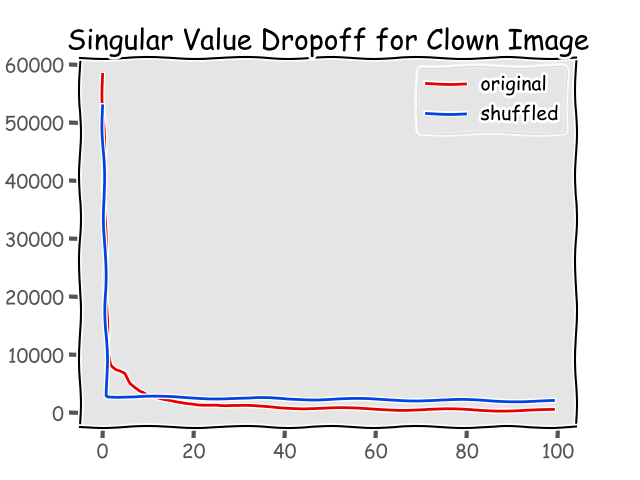
\includegraphics[width = 4in]{hw6_starter_file/dropoff.png}
    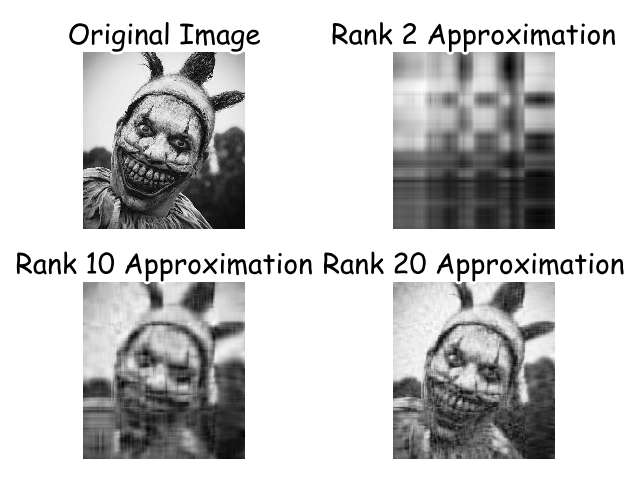
\includegraphics[width = 4in]{hw6_starter_file/reconstruction.png}
\end{center}
Pretty neat to be honest. It's encouraging that the eigenvalues of the dropoff drops off so much for the shuffled data. Makes sense logically but still neat. 
\end{solution}


\end{document}
